%%%%%%%%%%%%%%%%%%%%%%%%%% ch2-StochasticProcess
\begin{frame}[shrink]
\frametitle{ch2. Example}
\tableofcontents%[hideallsubsections]
\end{frame}

\section{习题}

\begin{frame}{均匀分布随机变量$x$的均值$\mu_x$和方差$\sigma_x^2$}
\begin{example}
求如图均匀分布随机变量$x$的均值$\mu_x$和方差$\sigma_x^2$。
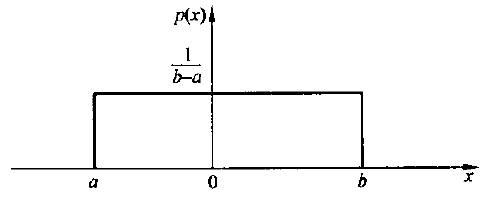
\includegraphics[scale=0.3]{ex2-1}
\end{example}
\end{frame}

\begin{frame}{均匀分布随机变量$x$的均值$\mu_x$和方差$\sigma_x^2$}
解: 随机变量$x$的概率密度函数$p(x)$为
\[p(x)=\begin{cases}
\frac{1}{b-1}, &a\le x\le b\\
0, &\text{其他}
\end{cases} \]

	根据随机变量均值的定义,有
	\begin{align*}
	\mu_x=E(x)&=\int_{-\infty}^{\infty}xp(x)dx=\int_{a}^{b}\frac{1}{b-1}p(x)dx =\frac{a+b}{2}
	\end{align*}
	根据随机变量方差的定义,有
	\begin{align*}
	\sigma_x^2=E[(x-\mu_x)^2]&=\int_{-\infty}^{\infty}(x-\mu_x)^2p(x)dx=\int_{a}^{b}\left(x-\frac{a+b}{2}\right)^2\frac{1}{b-a}dx \\
	&=\frac{(b-a)^2}{12}
	\end{align*}	
\end{frame}

\begin{frame}{高斯变量的线性组合仍然是高斯随机变量}
\begin{example}
	设随机变量$y$与$x$之间为线性关系$y=ax+b,a,b$为常数,且$a\ne 0$。已知随机变量$x$服从高斯分布,即
	\[p(x)=\left(\frac{1}{2\pi\sigma_x^2}\right)^{1/2}\exp\left[-\frac{(x-\mu_x)^2}{2\sigma_x^2}\right] \]
	证明随机变量$y$是服从均值为$a\mu_x+b$, 方差为$a^2\sigma_x^2$的高斯分布。
\end{example}
\end{frame}

\begin{frame}
\begin{proof}
	证法I: 雅可比变换法
	\begin{align*}
		&\text{因为}\qquad  y=ax+b \\
		&\text{所以,反函数为}\qquad  x=\frac{y-b}{a} \\
		&\text{且有}\qquad  \frac{dx}{dy}=\frac{1}{a} \\
		&\text{于是,由一维雅可比变换,得}  \\
		&p(y)=\left(\frac{1}{2\pi\sigma_x^2}\right)^{1/2}\exp\left[-\frac{(\frac{y-b}{a}-\mu_x)^2}{2\sigma_x^2}\right]\left|\frac{1}{a}\right| \\
		&=\left(\frac{1}{2\pi  a^2\sigma_x^2}\right)^{1/2}\exp\left[-\frac{(y-(a\mu_x+b))^2}{2a^2\sigma_x^2}\right]  
	\end{align*}
	所以,随机变量$y$是服从均值为$a\mu_x+b$, 方差为$a^2\sigma_x^2$的高斯分布。
\end{proof}
\end{frame}

\begin{frame}
\begin{proof}
	证法II: 利用高斯随机变量的特性来证明\\
	因为  $y=ax+b$ \\
	是高斯随机变量$x$的线性变换,所以$y$仍然是高斯随机变量。\\
	其均值$\mu_y$和方差$\sigma_y^2$分别为
	\begin{align*}
	\mu_y&=E(y)=E(ax+b)=aE(x)+b\\
	&=a\mu_x+b\\
	\sigma_y^2&=E[(y-\mu_y)^2]=E[(ax+b-a\mu_x-b)^2]\\
	&=a^2E[(x-\mu_x)^2]\\
	&=a^2\sigma_x^2
	\end{align*}
	所以,随机变量$y$是服从均值为$a\mu_x+b$, 方差为$a^2\sigma_x^2$的高斯分布。
\end{proof}
\end{frame}

\begin{frame}{周期性锯齿波}
\begin{example}
设随机过程的样本函数是周期性的锯齿波,下图是它的两个样本函数。各样本函数具有相同的波形,其区别在于锯齿波的起点位置不同。设在$t=0$后的第一个值位于$\tau,\tau$是一个随机变量,它在$(0,T)$上服从均匀分布。若锯齿波的幅度为常数$A$, 求该随机过程$x(t)$的一维概率密度函数。
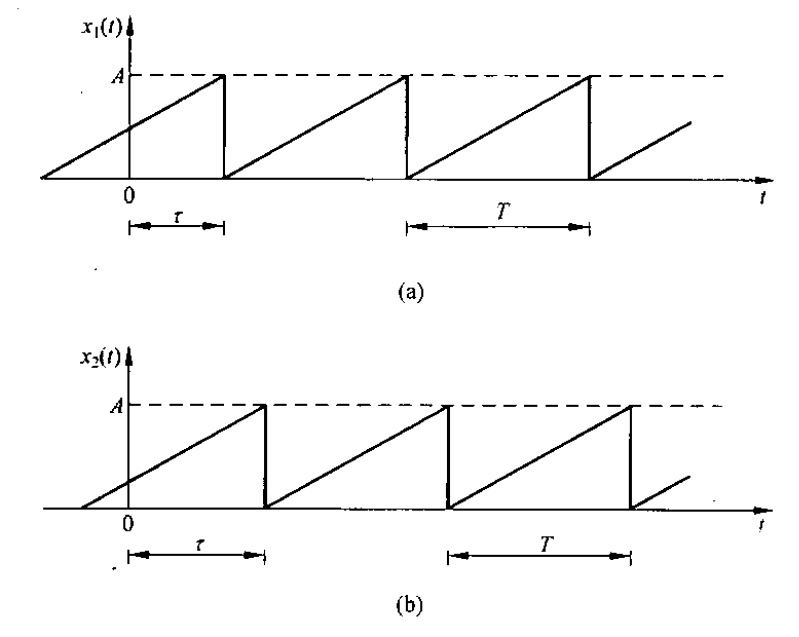
\includegraphics[scale=0.2]{ex2-11}
\end{example}
\end{frame}

\begin{frame}
解: 因为是周期性锯齿波, 所以只需求出一个周期的概率密度函数。
在一个周期内,随机信号为
\[x(t)=\frac{A}{T}(t+T-\tau),\quad t-T\le t\le\tau \]
其反函数$\tau$为
\[\tau=T-\frac{T}{A}x(t)+t,\quad 0\le\tau\le T,0\le x\le A \]
因为随机变量$\tau$在$(0,T)$上脉冲均匀分布,即
\[
p(\tau)=\begin{cases}
\frac{1}{T},&0\le\tau\le T\\
0,&\text{其它}
\end{cases} 
\]
所以,由一维雅可比变换,得
\begin{align*}
p(x;t)&=p[\tau=h(x)]\left|\frac{d\tau}{dx}\right|\\
&=\begin{cases}
\frac{1}{T}\frac{T}{A}\\
0
\end{cases}
=\begin{cases}
\frac{1}{A}, &0\le x\le A\\
0,&\text{其它}
\end{cases}
\end{align*}
\end{frame}

\begin{frame}{确知函数$a(t)$的均值$E[a(t)]=a(t)$}
\begin{example}
设随机过程$x(t)$的均值为$\mu_x(t)$,自相关函数为$r_x(t_j,t_k)$。若有随机过程$y(t)=a(t)x(t)x(t)+b(t)$, 其中$a(t),b(t)$是确知函数。求随机过程$y(t)$的均值和自相关函数。
\end{example}
\end{frame}

\begin{frame}{确知函数$a(t)$的均值$E[a(t)]=a(t)$}
解:\\
由均值定义$E[x(\xi)]\mathop{=}\limits^{def}\mu_x=\int_{-\infty}^{\infty}xp(x)dx$知:\\
确知函数$a(t)$的均值:
\begin{align*}
E[a(t)]&=\int_{-\infty}^{\infty}a(t)p(x)dx\\
&=a(t)\int_{-\infty}^{\infty}p(x)dx &&\text{by $a(t)$是常数}\\
&=a(t)\cdot 1 &&by \int_{-\infty}^{\infty}p(x)dx=1\\
&=a(t)
\end{align*}
\end{frame}

\begin{frame}{确知函数$a(t)$的均值$E[a(t)]=a(t)$}
解(续):随机过程$y(t)$的均值为:
\begin{align*}
\mu_y&=E[y(t)]=E[a(t)x(t)+b(t)]=E[a(t)x(t)]+E[b(t)]\\
&=a(t)E[x(t)]+b(t)=a(t)\mu_x+b(t)
\end{align*}
随机过程$y(t)$的自相关函数为:
\begin{align*}
\r_y(t_j,t_k)&=E[y(t_j)y(t_k)]\\
&=E[(a(t_j)x(t_j)]+b(t_j))(a(t_k)x(t_k)+b(t_k))]\\
&=a(t_j)a(t_k)E[x(t_j)]x(t_k)]+a(t_j)b(t_k)E[x(t_j)]+b(t_j)a(t_k)E[x(t_k)]+b(t_j)b(t_k)\\
&=a(t_j)a(t_k)r_x(t_j,t_k)+a(t_j)b(t_k)\mu_x(t_j)+b(t_j)a(t_k)\mu_x(t_k)+b(t_j)b(t_k)
\end{align*}
其中: $\mu_x(t_k)=E[x(t_k)],r_x(t_j,t_k)=E[x(t_j)x(t_k)]$
\end{frame}

\begin{frame}{平稳随机过程随着间隔的增大,采样之间的相关性减小}
\begin{example}
	对于平稳随机过程$x(t)$, 随着间隔$\tau$的增大,随机过程采样之间的相关性减小,即满足
	\[\lim\limits_{\tau\to\infty}c_x(\tau)=0 \]
	证明: (1) $r_x(\infty)=\mu_x^2$;\qquad  (2) $r_x(0)-r_x(\infty)=\sigma_x^2$
\end{example}
\end{frame}

\begin{frame}[shrink]
\begin{proof}
	(1) 因为 
		$$r_x(\tau)=c_x(\tau)+\mu_x^2$$
		所以
		$$\lim\limits_{\tau\to\infty}r_x(\tau)=\lim\limits_{\tau\to\infty}c_x(\tau)+\mu_x^2$$
		当
		$$\lim\limits_{\tau\to\infty}c_x(\tau)=0$$
		时,有
		$$\lim\limits_{\tau\to\infty}r_x(\tau)=r_x(\infty)=\mu_x^2$$
	(2) 因为
		$$r_x(0)=E[x(t)x(t)]=E[x^2(t)] $$
		而
		$$r_x(\infty)=\mu_x^2$$
		于是
		$$r_x(0)-r_x(\infty)=E[x^2(t)]-\mu_x^2=\sigma_x^2$$
\end{proof}
\end{frame}

\begin{frame}{周期性平稳过程的自相关函数也是周期性,且周期相同}
\begin{example}
	假定平稳随机过程$x(t)$是周期的, 周期为$T$, 即
	\[x(t)=x(t+T) \]
	证明其自相关函数$r_x(\tau)$也是以$T$为周期的, 即
	\[r_x(\tau)=r_x(\tau+T) \]
\end{example}
\end{frame}

\begin{frame}{周期性平稳过程的自相关函数也是周期性,且周期相同}
\begin{example}
	假定平稳随机过程$x(t)$是周期的, 周期为$T$, 即
	\[x(t)=x(t+T) \]
	证明其自相关函数$r_x(\tau)$也是以$T$为周期的, 即
	\[r_x(\tau)=r_x(\tau+T) \]
\end{example}
\begin{proof}
因为
\begin{align*}
r_x(\tau)&=E[x(t)x(t+\tau)]\\
&=E[x(t)x(t+\tau+T)]&& \text{by } x(t+\tau)=x(t+\tau+T)\\
&=r_x(\tau+T)
\end{align*}
\end{proof}
\end{frame}

\begin{frame}{联合平稳的随机过程}
\begin{example}
	设$x(t)$和$y(t)$是联合平稳的随机过程, 试证明:
	\begin{enumerate}
		\item $r_{xy}(\tau)=r_{yx}(-\tau),c_{xy}(\tau)=c_{yx}(-\tau)$
		\item $|r_{xy}(\tau)|^2\le r_x(0)r_y(0)$
		\item $|\rho_{xy}(\tau)\le 1$
	\end{enumerate}
\end{example}
\end{frame}

\begin{frame}{联合平稳的随机过程}
\begin{proof}
	\begin{enumerate}
		\item \begin{align*}
		r_{xy}(\tau)&=E[x(t)y(t+\tau)]=E[y(t+\tau)x(t)]=r_{xy}(-\tau)\\
		c_xy(\tau)&=E[(x(t)-\mu_x(t))(y(t+\tau)-\mu_y(t+\tau))]\\
		&=E[(y(t+\tau)-\mu_y(t+\tau))(x(t)-\mu_x(t))]\\
		&=c_{yx}(-\tau)
		\end{align*}
		\item \begin{align*}
		|r_{xy}(\tau)|^2&=|E[x(t)y(t+\tau)]|^2\le (E|x(t)y(t+\tau)|)^2\\
		&\le E|x(t)|^2E|y(t+\tau)|^2=r_x(0)r_y(0)
		\end{align*}
	\end{enumerate}
\end{proof}
\end{frame}

\begin{frame}{联合平稳的随机过程}
\begin{proof}
	\begin{enumerate}
		\setcounter{enumi}{2} %设定起始编号 
		\item 因为 
		\begin{align*}
		|c_{xy}(\tau)|^2&=|E[(x(t)-\mu_x(t))(y(t+\tau)-\mu_y(t+\tau))]|^2\\
		&\le E|(x(t)-\mu_x(t))|^2E|(y(t+\tau)-\mu_y(t+\tau))|^2\\
		&=c_x(0)c_y(0)=\sigma_x^2\sigma_y^2
		\end{align*}
		所以 
		\[|c_{xy}(\tau)|\le\sigma_x\sigma_y \]
		从而得
		\[|\rho_{xy}(\tau)|=\frac{|c_{xy}(\tau)|}{\sigma_x\sigma_y}\le 1 \]
	\end{enumerate}
\end{proof}
\end{frame}

\begin{frame}{雷达回波信号}
\begin{example}
	设$s(t)$是雷达的发射信号, 遇到目标后的反射信号为$as(t-t_0), t_0$是信号返回的延迟时间。如果回波信号中伴有加性噪声$n(t)$, 则接收到的信号为
	\[x(t)=as(t-t_0)+n(t) \]
	\begin{enumerate}
		\item 假定$s(t)$和$n(t)$是平稳相关的, 试求互相关函数$r_sx(\tau)$。
		\item 如果噪声$n(t)$的均值为零, 且与$s(t)$相互统计独立, 试求互相关函数$r_sx(\tau)$。
	\end{enumerate}
\end{example}
\end{frame}

\begin{frame}[shrink]
解:
	\begin{enumerate}
		\item 假定$s(t)$和$n(t)$是平稳相关的, 试求互相关函数$r_sx(\tau)$。\begin{align*}
		r_{xy}(\tau)&=E[s(t)x(t+\tau)] \\
		&=E[s(t)(as(t-t_0+\tau)+n(t+\tau)))] &&\text{by } x(t)=as(t-t_0)+n(t)\\
		&=aE[s(t)s(t-t_0+\tau)]+E[s(t)n(t+\tau)]\\
		&=ar_{s}(\tau-t_0)+r_{sn}(\tau)
		\end{align*}
		\item 如果噪声$n(t)$的均值为零, 且与$s(t)$相互统计独立, 试求互相关函数$r_sx(\tau)$。
		\begin{align*}
		r_{xy}(\tau)&=E[s(t)x(t+\tau)] \\
		&=E[s(t)(as(t-t_0+\tau)+n(t+\tau)))] &&\text{by } x(t)=as(t-t_0)+n(t)\\
		&=aE[s(t)s(t-t_0+\tau)]+E[s(t)n(t+\tau)] &&\text{确知信号$s(t)$看作常数}\\ 
		&=aE[s(t)s(t-t_0+\tau)]+s(t)E[n(t+\tau)] &&\text{by }E[n(t)]=0 \\
		&=ar_{s}(\tau-t_0)+r_{sn}(\tau)
		\end{align*}
	\end{enumerate}
\end{frame}

